\section{Method}
\label{sec:methodology}
PhyST-Net is an ExG-aware spatio-temporal graph Transformer designed for network-structured node forecasting with known external drivers and domain constraints. Given the inputs defined in Section~\ref{sec:problem_definition}, the model follows the pipeline in Fig.~\ref{fig:physt_architecture}. Historical target states and historical ExG are first embedded into node-level temporal representations. AGSP converts the temporal history into continuous tokens. A Transformer backbone learns temporal dependencies. R-STMF serves as a graph adapter that maps temporal node states to graph-enhanced node states. K-AMC injects future ExG into the latent representation. PI-DCH finally decodes the conditioned states into feasible forecasts respecting domain-specific bounds.

\begin{figure*}[!t]
\centering
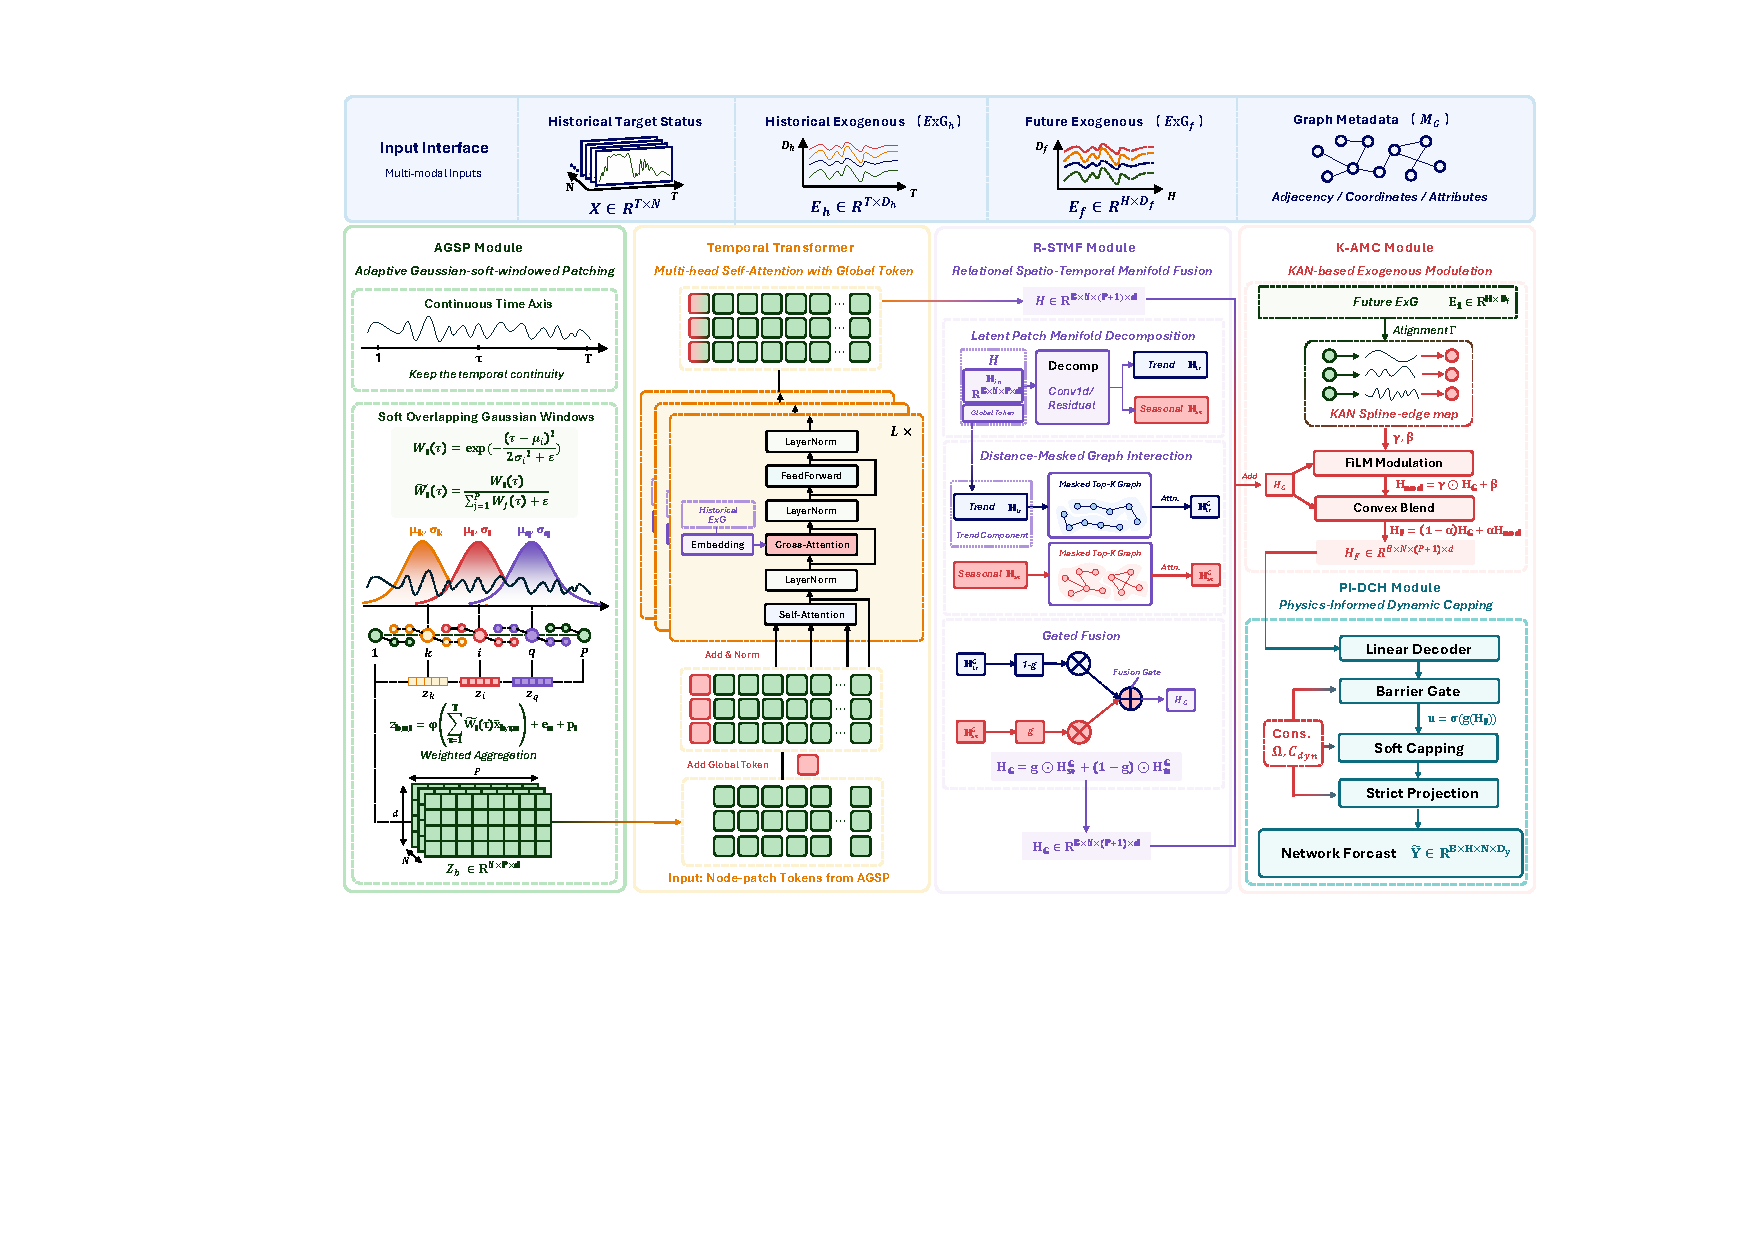
\includegraphics[width=\linewidth]{figures/Graph.pdf}
\caption{Overall architecture of PhyST-Net. The framework operates as an exogenous-aware vertical pipeline: (I) Multi-modal input interface; (II) AGSP continuous tokenization; (III) Transformer sequence encoding; (IV) R-STMF relational manifold fusion; (V) K-AMC spline-based conditioning; and (VI) PI-DCH domain-constrained forecasting. All external data (ExG and Metadata) and technical details are organized in peripheral tracks to ensure a clear and interpretable data flow.}
\label{fig:physt_architecture}
\end{figure*}


\subsection{Overall Framework}
\label{sec:overall_framework}
For a mini-batch, let $\mathbf{X}\in\mathbb{R}^{B\times T\times N\times D_x}$ denote historical target states, $\mathbf{E}^h\in\mathbb{R}^{B\times T\times D_h}$ denote historical ExG, and $\mathbf{E}^f\in\mathbb{R}^{B\times H\times D_f}$ denote future ExG. The model produces $\hat{\mathbf{Y}}\in\mathbb{R}^{B\times H\times N\times D_y}$. The computation can be written as
\begin{equation}
Z = \Phi_{patch}(\mathbf{X},\mathbf{E}^{h},M_G),
\label{eq:overall_patch}
\end{equation}
\begin{equation}
H_T = \Phi_{temp}(Z),\quad H_G = \Phi_{graph}(H_T,A,M_G),
\label{eq:overall_temp_graph}
\end{equation}
\begin{equation}
H_F = \Phi_{exg}(H_G,\mathbf{E}^{f}),\quad \hat{\mathbf{Y}} = \Phi_{head}(H_F,\mathbf{E}^{f},\Omega),
\label{eq:overall_exg_head}
\end{equation}
where $\Phi_{patch}$ is AGSP, $\Phi_{temp}$ is the temporal Transformer encoder, $\Phi_{graph}$ is the graph adapter (R-STMF), $\Phi_{exg}$ is future-ExG conditioning (K-AMC), and $\Phi_{head}$ is the physics-informed prediction head (PI-DCH). This decomposition emphasizes that the architectural backbone is defined on generic graph-structured sequences, while domain-specific knowledge is encapsulated in the input interface and the constraint head.

\subsection{Adaptive Gaussian-soft-windowed Patching}
\label{sec:agsp}
Transformer-based forecasters conventionally mitigate sequence length by aggregating observations into discrete temporal patches. While computationally convenient, fixed non-overlapping patches inevitably induce boundary artifacts when the underlying physical signal transverses a patch boundary. Aligning with emerging principles in complexity-balanced sequence modeling---where representational capacity is dynamically distributed proportional to signal variation---AGSP supersedes rigid patch assignments with learnable Gaussian soft-windows. This differentiable formulation empowers the architecture to autonomously allocate dense receptive fields to highly transient events and broader, smoother fields to stable operational regimes.

\begin{figure}[!t]
\centering
\begin{tikzpicture}[
    font=\rmfamily\scriptsize,
    >=Stealth,
    x=1.3cm, y=1.3cm,
    axis/.style={->, thick, draw=black!70},
    signal/.style={gray!70, thick},
    hard/.style={thick, fill opacity=0.15},
    soft/.style={thick, fill opacity=0.25},
    warn/.style={->, thick, draw=red!80!black},
    note/.style={font=\tiny, align=center}
]
    % (a) Rigid
    \begin{scope}[shift={(0, 2.1)}]
        \node[anchor=south west, font=\bfseries\small] at (0, 1.1) {Traditional Non-overlapping Hard Patches};
        \draw[axis] (0,0) -- (3.5,0) node[right] {Time $t$};
        \draw[signal] plot[domain=0.2:3.2, samples=100] (\x,{0.4 + 0.2*sin(deg(2*\x)) + 0.08*sin(deg(12*\x))});
        
        \draw[blue!70!black, hard, fill=blue!20] (0.4, 0) rectangle (1.2, 0.85);
        \draw[orange!85!black, hard, fill=orange!20] (1.2, 0) rectangle (2.0, 0.85);
        \draw[green!60!black, hard, fill=green!20] (2.0, 0) rectangle (2.8, 0.85);
        
        \node[text=red!80!black, font=\bfseries\scriptsize, align=center] (art1) at (1.6, 1.15) {Temporal Discontinuity};
        \draw[warn] (1.4, 1.05) -- (1.2, 0.9);
        \draw[warn] (1.8, 1.05) -- (2.0, 0.9);
    \end{scope}
    
    % (b) Soft
    \begin{scope}[shift={(0, 0)}]
        \node[anchor=south west, font=\bfseries\small] at (0, 1.1) {Proposed Adaptive Gaussian Soft Windows};
        \draw[axis] (0,0) -- (3.5,0) node[right] {Time $t$};
        \draw[signal] plot[domain=0.2:3.2, samples=100] (\x,{0.4 + 0.2*sin(deg(2*\x)) + 0.08*sin(deg(12*\x))});
        
        \path[fill=blue!30, draw=blue!80!black, soft] (0.2,0) plot[domain=0.2:1.8, samples=50] (\x,{0.85*exp(-((\x-1)^2)/0.15)}) -- (1.8,0) -- cycle;
        \node[blue!80!black, font=\scriptsize] at (1.0, 0.35) {$\mu_1, \sigma_1$};
        
        \path[fill=orange!30, draw=orange!90!black, soft] (0.8,0) plot[domain=0.8:2.4, samples=50] (\x,{0.7*exp(-((\x-1.6)^2)/0.1)}) -- (2.4,0) -- cycle;
        \node[orange!90!black, font=\scriptsize] at (1.6, 0.25) {$\mu_2, \sigma_2$};
        
        \path[fill=green!30, draw=green!60!black, soft] (1.4,0) plot[domain=1.4:3.0, samples=50] (\x,{0.95*exp(-((\x-2.2)^2)/0.2)}) -- (3.0,0) -- cycle;
        \node[green!60!black, font=\scriptsize] at (2.2, 0.45) {$\mu_3, \sigma_3$};
        
        \node[anchor=north, font=\scriptsize, text=black!80] at (1.6, -0.2) {$\sum_i \tilde{W}_i(\tau) = 1$};
    \end{scope}
\end{tikzpicture}
\caption{Mechanics of AGSP. By replacing discrete sequence chunking with continuous, differentiable density windows, the model autonomously mitigates boundary artifacts and preserves temporal continuity. Each soft window is parameterized by a learnable center $\mu_i$ and bandwidth $\sigma_i$, with overlapping weights dynamically normalized.}
\label{fig:agsp_detail}
\end{figure}

For node $n$ and temporal window $i$, the unnormalized weight at time index $\tau\in\{1,\ldots,T\}$ is
\begin{equation}
W_i(\tau)=\exp\left(-\frac{(\tau-\mu_i)^2}{2\sigma_i^2+\epsilon}\right),
\label{eq:agsp_window}
\end{equation}
where $\mu_i$ and $\sigma_i$ are learnable center and bandwidth parameters. To ensure numerical stability and valid window properties, we parameterize the bandwidth as $\sigma_i = \text{softplus}(\rho_i) + \delta$, where $\rho_i$ is the learnable parameter. The centers $\mu_i$ are initialized to uniform grid locations across the historical window to encourage an ordered temporal partition. The weights are normalized across $P$ windows:
\begin{equation}
\tilde{W}_i(\tau)=\frac{W_i(\tau)}{\sum_{j=1}^{P}W_j(\tau)+\epsilon}.
\label{eq:agsp_norm}
\end{equation}
Let $\bar{x}_{n}(\tau)$ denote the embedded historical state. The token for node $n$ and patch $i$ is
\begin{equation}
z_{n,i}=\psi\left(\sum_{\tau=1}^{T}\tilde{W}_i(\tau)\bar{x}_{n}(\tau)\right)+e_n+p_i,
\label{eq:agsp_token}
\end{equation}
where $\psi(\cdot)$ is a linear projection, $e_n$ is a node embedding, and $p_i$ is a temporal patch embedding.

\subsection{Temporal Representation Learning}
\label{sec:temporal_encoder}
Adopting the global token philosophy \cite{wang2024timexer} to facilitate efficient long-range context fusion, the token tensor $Z$ is concatenated with a learnable global token $z_{global} \in \mathbb{R}^{B \times N \times 1 \times d}$ for each node. This global token serves as a sequence-level memory bottleneck, aggregating the macroscopic temporal representation (e.g., shared external regimes or system-wide traffic trends) across all local patches. 

We denote the temporal encoding backbone as $\operatorname{STEnc}(\cdot)$. In PhyST-Net, rather than a naive standard Transformer, STEnc incorporates a targeted cross-attention mechanism. Specifically, within each encoder layer, the augmented node-wise token sequence $[Z \parallel z_{global}]$ first undergoes standard multi-head self-attention. Subsequently, to enrich the macro-trend representation with system-wide context, the global token uniquely cross-attends to the embedded historical exogenous features (e.g., SCADA and time-mark metadata), acting as an information sink:
\begin{equation}
z_{global}' = z_{global} + \operatorname{CrossAttention}(z_{global}, \mathbf{E}^h, \mathbf{E}^h).
\label{eq:cross_attention}
\end{equation}
This contextually enriched sequence is then processed through the feed-forward networks, yielding the final temporal representation:
\begin{equation}
H_T=\operatorname{STEnc}([Z \parallel z_{global}]), \quad H_T\in\mathbb{R}^{B\times N\times (P+1)\times d}.
\label{eq:temporal_encoder}
\end{equation}
Crucially, rather than discarding the global token post-encoding, PhyST-Net structurally leverages it to separate the node's state into two distinct manifolds: a local-variation patch state $U \triangleq H_{T,1:P}$ and a macro-trend global state $R \triangleq H_{T,P+1}$.

\subsection{Relational Spatio-Temporal Manifold Fusion (R-STMF)}
\label{sec:rstmf}
R-STMF serves as the graph adapter, specifically designed to capture the multi-modal spatial dependencies inherent in physical networks. Unlike conventional graph operators that treat node features as monolithic vectors, R-STMF recognizes that spatial interactions occur across different temporal scales within the latent space. To address this, we perform a \textbf{Latent Patch Manifold Decomposition}.

Let $H_{in} = H_T$ denote the input latent representation. For each node $n$, we apply a 1D depth-wise convolution along the patch dimension to extract the smoothed trend component $H_{tr}$, while the residual represents the seasonal (oscillatory) component $H_{se}$:
\begin{align}
H_{tr} &= \operatorname{GELU}(\operatorname{Conv1d}(H_{in})), \label{eq:rstmf_decomp_tr} \\
H_{se} &= H_{in} - H_{tr}. \label{eq:rstmf_decomp_se}
\end{align}

\begin{figure*}[!t]
\centering
\resizebox{\textwidth}{!}{%
\begin{tikzpicture}[
    font=\rmfamily\scriptsize,
    >=Stealth,
    x=1.0cm, y=1.0cm,
    module/.style={
        draw=black!75,
        rounded corners=3pt,
        thick,
        align=center,
        fill=white,
        inner sep=3pt
    },
    state/.style={
        module,
        fill=blue!5,
        draw=blue!75!black,
        minimum width=1.55cm,
        minimum height=0.50cm
    },
    branch/.style={
        module,
        fill=violet!5,
        draw=violet!75!black,
        minimum width=1.65cm,
        minimum height=0.50cm
    },
    graph/.style={
        module,
        fill=teal!5,
        draw=teal!70!black,
        minimum width=2.00cm,
        minimum height=0.78cm
    },
    mask/.style={
        module,
        fill=red!4,
        draw=red!75!black,
        dashed,
        minimum width=2.35cm,
        minimum height=0.58cm
    },
    op/.style={
        circle,
        draw=black!80,
        thick,
        fill=white,
        minimum size=6.0mm,
        inner sep=0pt
    },
    arrow/.style={
        ->,
        line width=0.90pt,
        draw=black!75
    },
    maskarrow/.style={
        ->,
        dashed,
        line width=0.80pt,
        draw=red!75!black
    },
    lab/.style={
        font=\tiny,
        fill=white,
        inner sep=1.1pt,
        text=black!80
    },
    title/.style={
        anchor=north west,
        font=\bfseries\scriptsize
    }
]

% ---------------------------------------------------------
% Canvas and background panels
% ---------------------------------------------------------
\path[use as bounding box] (-0.55,-0.85) rectangle (13.30,4.25);

\draw[fill=blue!2, draw=blue!15, rounded corners=4pt]
    (-0.35,-0.55) rectangle (3.25,4.00);
\node[title, text=blue!75!black] at (-0.25,3.90)
    {1. Latent Patch Decomposition};

\draw[fill=orange!2, draw=orange!18, rounded corners=4pt]
    (3.55,-0.55) rectangle (8.25,4.00);
\node[title, text=orange!85!black] at (3.65,3.90)
    {2. Distance-Masked Top-$K$ Graph Interaction};

\draw[fill=green!2, draw=green!18, rounded corners=4pt]
    (8.55,-0.55) rectangle (13.05,4.00);
\node[title, text=green!80!black] at (8.65,3.90)
    {3. Learnable Gated Fusion};

% ---------------------------------------------------------
% Stage 1: decomposition
% ---------------------------------------------------------
\node[state, fill=gray!6, draw=gray!75!black, minimum width=1.75cm]
    (hin) at (0.95,2.40) {\textbf{$H_{in}$}};

\node[module, minimum width=1.95cm, minimum height=0.82cm]
    (decomp) at (2.15,2.40)
    {\textbf{Decomposition}\\[-1pt]
    {\tiny Conv1D+GELU / residual}};

\node[branch] (htr) at (2.15,3.10)
    {\textbf{Trend} $H_{tr}$};

\node[branch] (hse) at (2.15,1.70)
    {\textbf{Seasonal} $H_{se}$};

\draw[arrow] (hin.east) -- (decomp.west);
\draw[arrow] (decomp.north) -- (htr.south);
\draw[arrow] (decomp.south) -- (hse.north);

\node[lab] at (1.75,0.65)
    {$H_{tr}=\mathrm{GELU}(\mathrm{Conv1D}(H_{in}))$};
\node[lab] at (1.75,0.35)
    {$H_{se}=H_{in}-H_{tr}$};

% ---------------------------------------------------------
% Stage 2: graph interaction
% ---------------------------------------------------------
\node[mask] (mask) at (5.95,3.35)
    {$\mathcal{M}_{dist}$ + branch-specific Top-$K$};

\node[graph] (gtr) at (5.30,2.75)
    {Masked Top-$K$\\[-1pt]
    Graph Prop. $\mathbf{A}_{tr}$};

\node[graph] (gse) at (5.30,1.45)
    {Masked Top-$K$\\[-1pt]
    Graph Prop. $\mathbf{A}_{se}$};

\node[state, fill=teal!3, draw=teal!70!black, minimum width=1.20cm]
    (hgtr) at (7.25,2.75) {$H_{tr}^{G}$};

\node[state, fill=teal!3, draw=teal!70!black, minimum width=1.20cm]
    (hgse) at (7.25,1.45) {$H_{se}^{G}$};

\draw[arrow] (htr.east) -- ++(0.55,0) |- (gtr.west);
\draw[arrow] (hse.east) -- ++(0.55,0) |- (gse.west);

\draw[arrow] (gtr.east) -- (hgtr.west);
\draw[arrow] (gse.east) -- (hgse.west);

% short mask injection arrows
\draw[maskarrow] (mask.south west) -- (gtr.north);
\draw[maskarrow] (mask.south east) -- (gse.north);

% ---------------------------------------------------------
% Stage 3: gated fusion
% ---------------------------------------------------------
\node[module, minimum width=1.80cm, minimum height=0.55cm]
    (gate) at (9.85,3.35)
    {Gate $\sigma(\cdot)$};

\node[op] (multr) at (9.80,2.75) {\Large $\otimes$};
\node[op] (mulse) at (9.80,1.45) {\Large $\otimes$};

\node[op] (add) at (11.05,2.10) {\Large $\oplus$};

\node[state, minimum width=2.25cm]
    (hg) at (12.15,2.10)
    {\textbf{$H_G$}};

\draw[arrow] (hgtr.east) -- (multr.west);
\draw[arrow] (hgse.east) -- (mulse.west);

\draw[arrow] (gate.south west) -- (multr.north)
    node[midway, left, lab] {$1-g$};

\draw[arrow] (gate.south east) -- (mulse.north)
    node[midway, right, lab] {$g$};

\draw[arrow] (multr.east) -- ++(0.38,0) |- (add.north);
\draw[arrow] (mulse.east) -- ++(0.38,0) |- (add.south);
\draw[arrow] (add.east) -- (hg.west);

\node[lab] at (10.95,0.65)
    {$H_G=g\odot H_{se}^{G}+(1-g)\odot H_{tr}^{G}$};

\end{tikzpicture}
}
\caption{Detailed architecture of R-STMF. The latent representation is decomposed into trend and seasonal manifolds. Each branch performs distance-masked Top-$K$ graph propagation with branch-specific routing, and the resulting graph-enhanced manifolds are fused through a learnable gate.}
\label{fig:rstmf_detail}
\end{figure*}

This decomposition ensures that the model can independently learn how macro-scale trends and micro-scale seasonal fluctuations propagate through the graph.

\subsubsection{Distance-Masked Relational Pruning}
For each manifold $c \in \{se, tr\}$, we compute relational attention scores across nodes. To enforce physical realism and reduce computational overhead, we introduce a \textbf{Distance-Masked Top-$K$ Pruning} strategy. Given a physical distance matrix or prior topology, we define a binary mask $\mathcal{M}_{dist}$, where $\mathcal{M}_{ij}=1$ only if node $j$ is within a feasible interaction radius of node $i$. The masked attention score $S_c$ is:
\begin{equation}
\resizebox{0.88\hsize}{!}{$
S_{c,ij} = \begin{cases} \frac{Q_c(K_c)^{\top}}{\sqrt{d_m}} & \text{if } \mathcal{M}_{ij}=1 \\ -\infty & \text{otherwise} \end{cases}, \quad A_c=\operatorname{Softmax}\left(\operatorname{TopK}(S_c, K_c)\right).
$}
\label{eq:rstmf_routing}
\end{equation}
Subsequently, we perform Top-$K$ selection on the remaining scores to ensure a sparse and robust graph routing. Finally, the graph-enhanced seasonal and trend manifolds are recombined using a learnable gated fusion mechanism:
\begin{align}
g &= \sigma(\operatorname{Linear}([H_{se}^G \parallel H_{tr}^G])), \\
H_G &= g \odot H_{se}^G + (1-g) \odot H_{tr}^G,
\label{eq:rstmf_fusion}
\end{align}
where $H_{c}^G$ denotes the manifold $c$ after spatial propagation via $A_c$. This dual-branch architecture allows PhyST-Net to model complex spatio-temporal interactions without conflating multi-resolution physical mechanisms.

\subsection{Future-ExG Conditioning (K-AMC)}
\label{sec:kamc}
We refer to this module as K-AMC, short for KAN-enhanced Adaptive Modulation and Conditioning. It serves as a generalized interface for known systemic drivers, injecting future exogenous drivers $\mathbf{E}^f \in \mathbb{R}^{B \times H \times D_f}$ into the latent representations. Aligning with the TimeXer philosophy \cite{wang2024timexer}, the macro-trend global token acts as the primary bridge to cross-attend and ingest external factors. We define an alignment operator $\Gamma$ that maps the future horizon into variate tokens corresponding to the latent states.

\begin{figure*}[!t]
\centering
\resizebox{\textwidth}{!}{%
\begin{tikzpicture}[
    font=\rmfamily\scriptsize,
    >=Stealth,
    x=1.15cm, y=1.00cm,
    module/.style={
        draw=black!75,
        rounded corners=3pt,
        thick,
        align=center,
        fill=white,
        inner sep=3pt
    },
    input/.style={
        module,
        fill=blue!5,
        draw=blue!75!black,
        minimum width=2.10cm,
        minimum height=0.52cm
    },
    process/.style={
        module,
        fill=gray!5,
        draw=black!65,
        minimum width=2.15cm,
        minimum height=0.58cm
    },
    kan/.style={
        module,
        fill=teal!5,
        draw=teal!70!black,
        minimum width=1.75cm,
        minimum height=1.05cm
    },
    param/.style={
        module,
        fill=violet!5,
        draw=violet!75!black,
        minimum width=1.35cm,
        minimum height=0.48cm
    },
    film/.style={
        module,
        fill=orange!6,
        draw=orange!85!black,
        minimum width=2.65cm,
        minimum height=0.95cm
    },
    blend/.style={
        module,
        fill=orange!4,
        draw=orange!85!black,
        dashed,
        minimum width=3.15cm,
        minimum height=0.95cm
    },
    arrow/.style={
        ->,
        line width=0.9pt,
        draw=black!75
    },
    auxarrow/.style={
        ->,
        line width=0.85pt,
        draw=black!55
    },
    residual/.style={
        ->,
        line width=0.95pt,
        draw=gray!75
    },
    title/.style={
        anchor=north west,
        font=\bfseries\scriptsize
    },
    note/.style={
        font=\tiny,
        align=center,
        text=black!75
    }
]

% ---------------------------------------------------------
% Canvas and background panels
% ---------------------------------------------------------
\path[use as bounding box] (-0.45,-0.65) rectangle (12.55,4.20);

\draw[fill=blue!2, draw=blue!15, rounded corners=4pt]
    (-0.30,-0.45) rectangle (3.05,3.95);
\node[title, text=blue!75!black] at (-0.20,3.85)
    {1. ExG Parameter Generation};

\draw[fill=teal!2, draw=teal!15, rounded corners=4pt]
    (3.35,-0.45) rectangle (7.35,3.95);
\node[title, text=teal!70!black] at (3.45,3.85)
    {2. FiLM Modulation};

\draw[fill=orange!2, draw=orange!18, rounded corners=4pt]
    (7.65,-0.45) rectangle (12.35,3.95);
\node[title, text=orange!85!black] at (7.75,3.85)
    {3. Stable Blending};

% ---------------------------------------------------------
% Stage 1: ExG parameter generation
% ---------------------------------------------------------
\node[input] (ef) at (1.35,3.20)
    {\textbf{Future ExG} $\mathbf{E}^{f}$};

\node[process] (align) at (1.35,2.35)
    {Alignment $\Gamma$\\[-1pt]
    {\tiny AvgPool1d to $P$ patches}};

\node[kan] (kanblk) at (1.35,1.35) {};

\node[font=\bfseries\scriptsize] at (1.35,1.70) {KAN};
\node[note] at (1.35,1.50) {spline edges};

% compact KAN internal edge diagram
\coordinate (u1) at (1.00,1.30);
\coordinate (u2) at (1.70,1.30);
\coordinate (v1) at (1.00,1.02);
\coordinate (v2) at (1.70,1.02);

\fill[violet!85!black] (u1) circle (1.15pt);
\fill[violet!85!black] (u2) circle (1.15pt);
\fill[violet!85!black] (v1) circle (1.15pt);
\fill[violet!85!black] (v2) circle (1.15pt);

\draw[violet!80!black, line width=0.75pt] (u1) -- (v1);
\draw[violet!80!black, line width=0.75pt] (u2) -- (v2);
\draw[violet!80!black, line width=0.75pt] (u1) -- (v2);
\draw[violet!80!black, line width=0.75pt] (u2) -- (v1);

\node[violet!80!black, font=\tiny, fill=teal!5, inner sep=1pt]
    at (1.35,1.16) {$\phi$};

\node[param] (params) at (1.35,0.45)
    {$[\gamma,\beta]$};

\draw[arrow] (ef.south) -- (align.north);
\draw[arrow] (align.south) -- (kanblk.north);
\draw[arrow] (kanblk.south) -- (params.north);

% ---------------------------------------------------------
% Stage 2: FiLM modulation
% ---------------------------------------------------------
\node[input, fill=gray!8, draw=gray!75!black, minimum width=1.65cm]
    (hg) at (4.75,2.85) {\textbf{$H_G$}};

\node[film] (film) at (5.35,1.55)
    {\textbf{FiLM Modulation}\\[2pt]
    $H_{\mathrm{mod}}=\gamma\odot H_G+\beta$};

\node[module, fill=orange!8, draw=orange!85!black, minimum width=1.55cm]
    (hmod) at (6.95,1.55) {\textbf{$H_{\mathrm{mod}}$}};

\draw[arrow] (hg.south) |- (film.north);
\draw[auxarrow] (params.east) -- ++(1.10,0) |- (film.west);
\draw[arrow] (film.east) -- (hmod.west);

% ---------------------------------------------------------
% Stage 3: Convex blending
% ---------------------------------------------------------
\node[blend] (blend) at (9.20,1.55)
    {\textbf{Convex Blend} $(\alpha=0.1)$\\[2pt]
    $H_F=(1-\alpha)H_G+\alpha H_{\mathrm{mod}}$};

\node[input, minimum width=2.95cm]
    (hf) at (11.30,1.55)
    {\textbf{ExG-conditioned State} $H_F$};

\draw[arrow] (hmod.east) -- (blend.west);
\draw[arrow] (blend.east) -- (hf.west);

% residual path from H_G to blend, routed above
\draw[residual] (hg.east) -- ++(3.05,0) |- (blend.north);
\node[note, fill=white, inner sep=1pt] at (8.25,2.85)
    {residual $H_G$};

\end{tikzpicture}
}
\caption{Mechanics of K-AMC. Future exogenous drivers are aligned to the patch scale and processed by a compact KAN block to generate dynamic modulation parameters. The graph-enhanced state is first modulated by FiLM and then stabilized through convex blending with the original state.}
\label{fig:kamc_detail}
\end{figure*}

The aligned representation $\bar{\mathbf{E}}^f$ is then passed through a Kolmogorov-Arnold Network (KAN) block. Unlike standard MLPs, KANs parameterize transformations using learnable univariate B-spline functions on the edges. For an input feature $x$, the edge function is defined as:
\begin{equation}
\phi(x) = w_b \operatorname{SiLU}(x) + \sum_{i=1}^{k} c_i B_i(x),
\label{eq:kan_edge_sum}
\end{equation}
where $B_i(x)$ are B-spline basis functions. The analytical derivative is:
\begin{equation}
\frac{\partial \phi(x)}{\partial x} = w_b \operatorname{SiLU}'(x) + \sum_{i=1}^{k} c_i B'_i(x).
\label{eq:kan_derivative}
\end{equation}
By aggregating these edge functions, the KAN block produces modulation parameters $[\gamma,\beta]=\operatorname{KAN}(\bar{\mathbf{E}}^f)$. The final conditioned latent state is then obtained via element-wise scale and shift, stabilized by a convex blending scheme with hyperparameter $\alpha=0.1$:
\begin{equation}
H_{mod} = \gamma \odot H_G + \beta, \quad H_F = (1-\alpha)H_G + \alpha H_{mod}.
\label{eq:kamc_mod}
\end{equation}

\subsection{Physics-Informed Dynamic Capping Head (PI-DCH)}
\label{sec:pidch}
PI-DCH instantiates the constraint operator $\mathcal{C}_{\Omega}$. In mission-critical environments such as smart grids, safety-critical traffic routing, and industrial control systems, deploying predictive models mandates rigorous output-space guidance to preclude physically unfeasible trajectories. While hard projection operators (e.g., clipping) guarantee bounded outputs, they may create a mismatch between training and inference, and can severely weaken gradient signals when used naively, hampering the learning process.

To ensure that the model remains physically consistent even under extreme scenarios, we adopt a dual-stage enforcement strategy. While $\hat{Y}_{soft}=\tilde{Y}+u\odot(C_{dyn}-\tilde{Y})$ provides the differentiable path necessary for optimization via a learned barrier gate $u=\sigma(g(H_F))$, we define the final deployment-ready forecast $\hat{\mathbf{Y}}$ through a \textbf{Strict Operational Boundary Enforcement} layer:
\begin{equation}
\hat{\mathbf{Y}} = \operatorname{Proj}_{\mathcal{K}}(\hat{Y}_{soft}) \triangleq \max(0, \min(\hat{Y}_{soft}, C_{dyn})),
\label{eq:pidch_enforcement}
\end{equation}
where $\operatorname{Proj}_{\mathcal{K}}$ denotes the Euclidean projection onto the dynamic feasible set $\mathcal{K} = [0, C_{dyn}]$. Crucially, this projection is treated as a non-trainable safety layer during inference to guarantee 100\% compliance with physical limits. By decoupling the differentiable steering ($\hat{Y}_{soft}$) from the strict enforcement ($\hat{\mathbf{Y}}$), PhyST-Net achieves the dual goals of stable gradient backpropagation and absolute operational feasibility.

\subsection{Computational Complexity Analysis}
\label{sec:complexity_analysis}
A core motivation of PhyST-Net is mitigating the severe computational bottlenecks of dense spatio-temporal Transformers, which conventionally exhibit a time complexity of $\mathcal{O}(N \cdot T^2 + T \cdot N^2)$ for sequence length $T$ and node count $N$. PhyST-Net structurally resolves this through its decoupled topology.

In the temporal pathway, the AGSP module compresses the raw $T$-length sequence into $P$ continuous tokens (where $P \ll T$). Consequently, the temporal Transformer encoder's self-attention complexity is reduced from $\mathcal{O}(N \cdot T^2)$ to $\mathcal{O}(N \cdot P^2)$. 

In the spatial pathway, standard full-graph attention requires $\mathcal{O}(P \cdot N^2)$ operations. The R-STMF module introduces a Top-$K$ sparse masking strategy (Eq.~\ref{eq:rstmf_routing}), restricting message passing to a parameterized neighborhood size $K$. This bounds the spatial complexity to $\mathcal{O}(P \cdot K \cdot N)$. Thus, the overall self-attention complexity of the PhyST-Net backbone is decoupled and bounded by $\mathcal{O}(N \cdot P^2 + P \cdot K \cdot N)$, rendering the architecture highly scalable for large physical networks and extended forecasting horizons without sacrificing expressive capability.

\subsection{Optimization Objective}
\label{sec:optimization}
To bridge the gap between purely data-driven forecasting and physical feasibility, we minimize a multi-objective loss $\mathcal{L} = \mathcal{L}_{mae} + \lambda_{\Omega}\mathcal{L}_{penalty}$. The penalty term $\mathcal{L}_{penalty}$ structurally regularizes the model to internalize the operational set $\Omega$ during backpropagation. Utilizing the positive-part operator $[x]^+ \triangleq \max(0, x)$, we decouple the penalty into two physically meaningful components: a non-negativity constraint and a dynamic capacity limit constraint:
\begin{align}
\mathcal{L}_{penalty} &= \mathcal{L}_{neg} + \mathcal{L}_{cap}, \label{eq:feasibility_penalty_total} \\
\mathcal{L}_{neg} &= \frac{1}{|\mathcal{D}|HN} \sum_{\mathcal{D}} \sum_{n,h} [-\hat{Y}_{soft,n,h}]^+, \label{eq:feasibility_penalty_neg} \\
\mathcal{L}_{cap} &= \frac{1}{|\mathcal{D}|HN} \sum_{\mathcal{D}} \sum_{n,h} [\hat{Y}_{soft,n,h} - C_{dyn,n,h}]^+. \label{eq:feasibility_penalty_cap}
\end{align}
This decoupled formulation ensures the model learns to respect physical boundaries natively, thereby reducing the reliance on reactive clipping at inference time. The overall training logic is summarized in Algorithm~\ref{alg:physt_net}.

\begin{algorithm}[!t]
\caption{PhyST-Net Forward Pass}
\label{alg:physt_net}
\begin{algorithmic}[1]
\REQUIRE Input tuple $\mathcal{X}_t = (\mathbf{X}, \mathbf{E}^h, \mathbf{E}^f, A, M_G)$, Domain knowledge $\Omega$.
\ENSURE Feasible network forecast $\hat{\mathbf{Y}}$.

\STATE \COMMENT{\textit{Phase I: AGSP Continuous Tokenization}}
\STATE Initialize learnable Gaussian parameters $\mu_i, \sigma_i$ for $P$ tokens using metadata $M_G$.
\FOR{each token $i \in \{1,\ldots,P\}$}
    \STATE Compute soft-window weights $W_i(\tau) = \exp\left(-\frac{(\tau-\mu_i)^2}{2\sigma_i^2+\epsilon}\right)$.
    \STATE Aggregate $\mathbf{X}$ and $\mathbf{E}^h$ via $W_i(\tau)$ to form continuous token $Z_{:,i,:}$.
\ENDFOR

\STATE \COMMENT{\textit{Phase II: Temporal Encoding ($\mathcal{H}_\theta$ part 1)}}
\STATE Process $Z$ via Multi-Head Self-Attention to capture temporal dependencies $\to H_T$.

\STATE \COMMENT{\textit{Phase III: R-STMF Graph Adaptation ($\mathcal{H}_\theta$ part 2)}}
\STATE Decompose $H_{in} = H_T$ into seasonal $H_{se}$ and trend $H_{tr}$ manifolds.
\STATE Apply Top-$K$ sparse masking to $A$ based on spatial similarities and physical distances.
\STATE Propagate $H_{se}$ and $H_{tr}$ over the masked graph and fuse $\to H_G$.

\STATE \COMMENT{\textit{Phase IV: K-AMC Exogenous Modulation ($\mathcal{H}_\theta$ part 3)}}
\STATE Align horizon-wise $\mathbf{E}^f$ to patch-wise representation $\bar{\mathbf{E}}^f$.
\STATE Compute B-spline edge functions via KAN block to generate $[\gamma, \beta]$.
\STATE Modulate latent states: $H_F \leftarrow (1-\alpha)H_G + \alpha(\gamma \odot H_G + \beta)$.

\STATE \COMMENT{\textit{Phase V: PI-DCH Constraint Decoding ($\mathcal{C}_\Omega$)}}
\STATE Decode unconstrained prediction $\tilde{Y} = \operatorname{Linear}(H_F)$.
\STATE Shape prediction softly: $\hat{Y}_{soft} \leftarrow \tilde{Y} + u \odot (C_{dyn} - \tilde{Y})$.
\STATE Project to feasible set: $\hat{\mathbf{Y}} \leftarrow \operatorname{Proj}_{\mathcal{K}}(\hat{Y}_{soft})$.

\RETURN $\hat{\mathbf{Y}}$.
\end{algorithmic}
\end{algorithm}
